\documentclass{beamer}

\usepackage{verbatim}
\usepackage{fancyvrb}
\usepackage{amsmath}
\usepackage{mathtools}
\usepackage{booktabs}
\usepackage{amssymb}
\usepackage{graphicx}
\usepackage{calc}
\usepackage{color}
\usepackage{multicol}
\usepackage{wrapfig}
\usepackage{natbib}
\usepackage[ruled,vlined]{algorithm2e}
\usepackage{animate}
\usepackage{mathtools}
\usepackage{listings}
\usepackage{xfrac}

% two col: two columns
\newenvironment{twocol}[4]{
\begin{columns}[c]
\column{#1\textwidth}
#3
\column{#2\textwidth}
#4
\end{columns}
}

\makeatletter
\setbeamertemplate{theorem begin}
{%
\begin{\inserttheoremblockenv}
  {}{\usebeamerfont*{block title}\usebeamercolor[fg]{block title}%
  \inserttheoremname
  %\inserttheoremnumber
  \ifx \inserttheoremaddition \empty \else\ (\inserttheoremaddition)\fi
  \inserttheorempunctuation}
  \normalfont
  }
  \setbeamertemplate{theorem end}{\end{\inserttheoremblockenv}}
\makeatother

\newcommand{\E}{\mathrm{E}}
\newcommand{\Var}{\mathrm{Var}}
\newcommand{\Cov}{\mathrm{Cov}}
\newcommand{\s}{\mathrm{s}}
\newcommand{\Corr}{\mathrm{Corr}}
\newcommand{\rank}{\mathrm{rank}}
\newcommand{\nullspace}{\mathrm{null}}
\newcommand{\myspan}{\mathrm{span}}
\DeclareMathOperator*{\argmax}{arg\,max}
\DeclareMathOperator*{\argmin}{arg\,min}
\DeclareMathOperator*{\softmax}{softmax}

\definecolor{darkgreen}{rgb}{0,0.5,0}

\newtheorem{prop}[theorem]{Proposition}
\newtheorem{exe}{Exercise}
\newtheorem{remark}{Remark}
\newtheorem{myproof}{Proof}

\definecolor{darkgreen}{rgb}{0,0.5,0}

\title{Diagnostics and Remedial Measures}
\author{Zhenisbek Assylbekov}
\institute{Department of Mathematics}
\date{Regression Analysis}

\AtBeginSection[]
{
  \begin{frame}<beamer>
    \tableofcontents[currentsection]
  \end{frame}
}

\begin{document}

\begin{frame}
  \titlepage
\end{frame}

\section{Diagnostics for Predictor Variable}

\begin{frame}{Diagnostics for Predictor Variable}
Goal: identify any outlying values that could affect the appropriateness of the linear model.
\vspace{10pt}

\pause Two main issues:
\begin{itemize}
    \item \pause Outliers (recall Extrapolation)
    \item \pause Dependence b/w $x_i$ and $i$
\end{itemize}
\vspace{10pt}

\pause To check these we use
\begin{itemize}
    \item Histogram and/or Boxplot
    \item Sequence plot
\end{itemize}
\end{frame}


\begin{frame}{Example}
{\color{blue}\url{https://raw.githubusercontent.com/zh3nis/MATH440/main/chp03/diag_x.R}}
\begin{center}
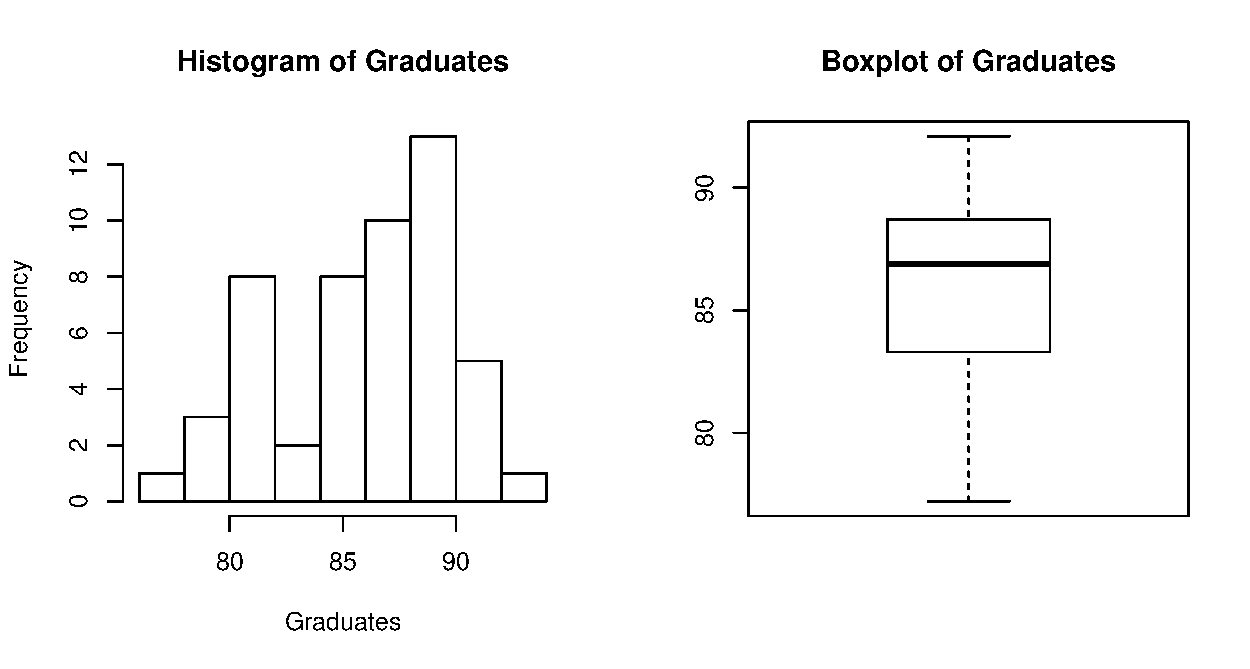
\includegraphics[width=.65\textwidth]{plots/hist_bp_x.pdf}\\
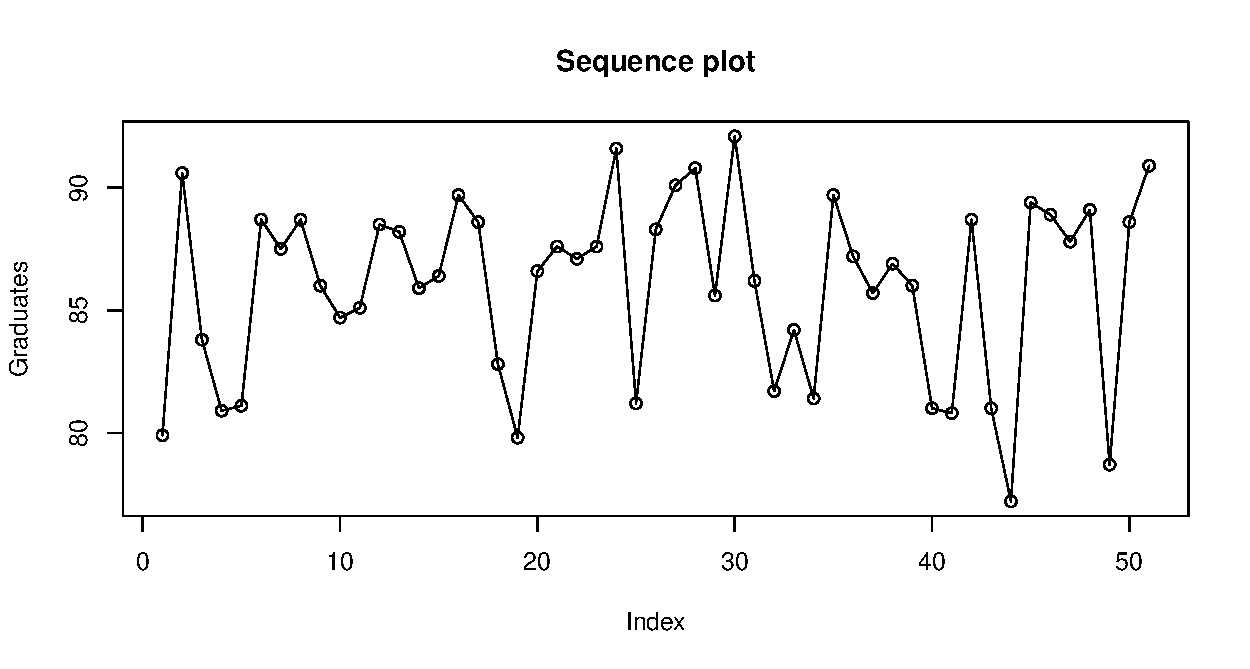
\includegraphics[width=.65\textwidth]{plots/seq_x.pdf}
\end{center}
\end{frame}

\section{Checking Assumptions}
\begin{frame}{Checking Assumptions}
Recall the SLR model:
\begin{align*}
&Y_i=\beta_0+\beta_1 x_i+\epsilon_i,\qquad i=1,\ldots,n\\
&\epsilon_i\,\,{\stackrel{\text{iid}}{\sim}}\,\,\mathcal{N}(0,\sigma^2)
\end{align*}
\pause After the model is fit, but \textit{before} any inference or conclusions are made, the assumptions of the model need to be checked.

\vspace{10pt}
\pause Assumptions:
\begin{enumerate}
    \item\pause Normality
    \item\pause Homogeneity of variance
    \item\pause Linearity
    \item\pause Independence
\end{enumerate}
\vspace{10pt}
\pause The assumptions are checked using the residuals $e_i:=y_i-\hat{y}_i$. This process is sometimes referred to as \textbf{residual analysis}.
\end{frame}

\subsection{Graphical Methods}
\begin{frame}[fragile]{Graphical Methods: Normality}{Normal Q-Q Plot}
\begin{itemize}
    \item The \textbf{empirical c.d.f.} for a r.s. $Y_1,\ldots,Y_n$ is given by $\hat{F}(y)=\frac{\#(Y_i\le y)}{n}=\frac1n\sum_i\mathbb{I}[Y_i\le y]$.
    \item \pause To compare an empirical distribution $\hat{F}(y)$ against some theoretical distribution $G(y)$, we can scatterplot quantiles $\hat{F}^{-1}(p)$ vs $G^{-1}(p)$ for $p\in[0,1]$. \pause This is called \textbf{Q-Q plot}.
\end{itemize} 
\pause
\begin{columns}
\begin{column}{.5\textwidth}
Comparing the distribution of poverty rates vs normal distribution using a Q-Q Plot.\\~\\
\begin{footnotesize}
{\color{blue}\url{https://raw.githubusercontent.com/zh3nis/MATH440/main/chp03/qq.R}}
\end{footnotesize}
\end{column}
\begin{column}{.5\textwidth}
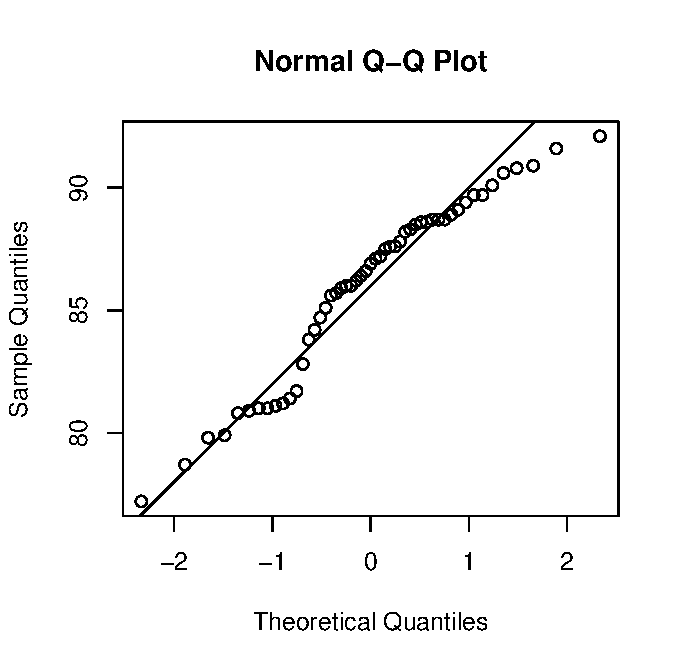
\includegraphics[width=\textwidth]{plots/qq_pov.pdf}
\end{column}
\end{columns}
\end{frame}

\begin{frame}{Graphical Methods: Normality}{Q-Q Plot for Residuals}

Recall, that by SLR assumtions, $\epsilon_i\,\,{\stackrel{\text{iid}}{\sim}}\,\,\mathcal{N}(0,\sigma^2)$. \pause In addition to checking normality of $y_i$'s, we should also check normality of the residuals $e_i$ once the model is fit.
\pause
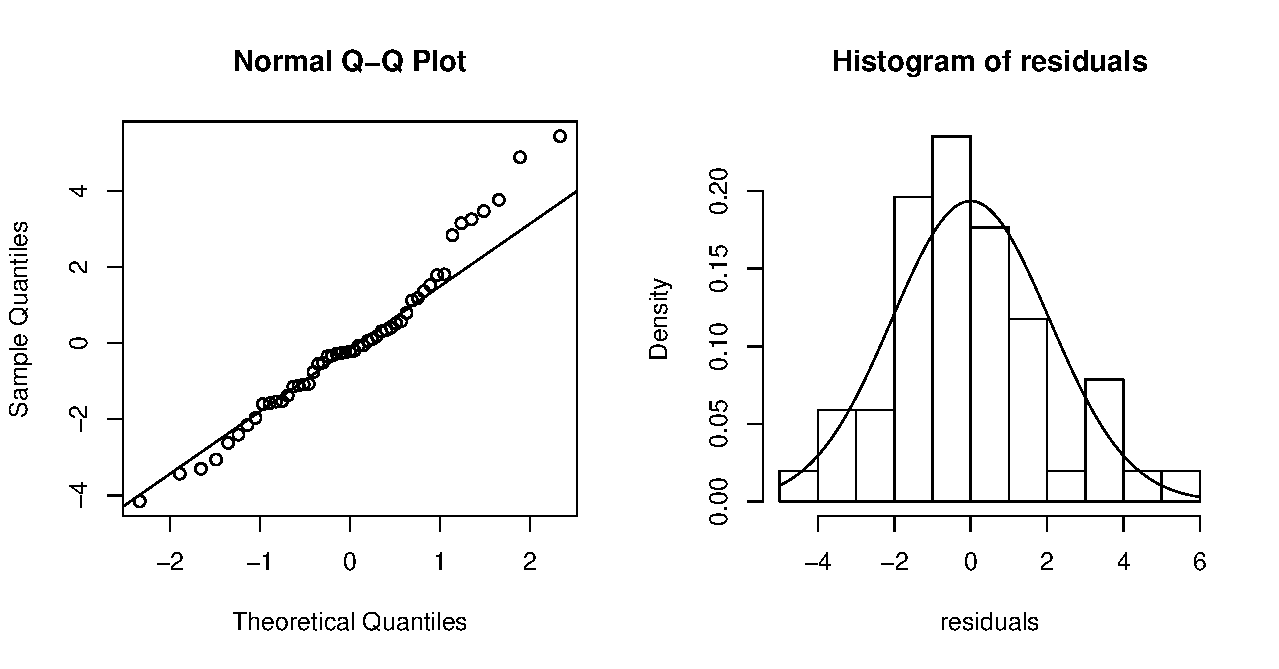
\includegraphics[width=\textwidth]{plots/res_qq_hist.pdf}\\
\footnotesize{\color{blue}\url{raw.githubusercontent.com/zh3nis/MATH440/main/chp03/res_plots.R}}
\end{frame}


\begin{frame}{Graphical Methods: Homogeneity of Variance / Linearity}
\begin{itemize}
    \item SLR assumes that $\Var[\epsilon_i]=\sigma^2$ is constant.
    \item<2->In order to check this assumption a plot of the residuals ($e_i$) versus the fitted values ($\hat{y}_i$) is used.
    \item<3->We expect to see a constant spread/distance of the residuals to the 0 line across all the $\hat{y}_i$ values.
    
\onslide<4->{\centerline{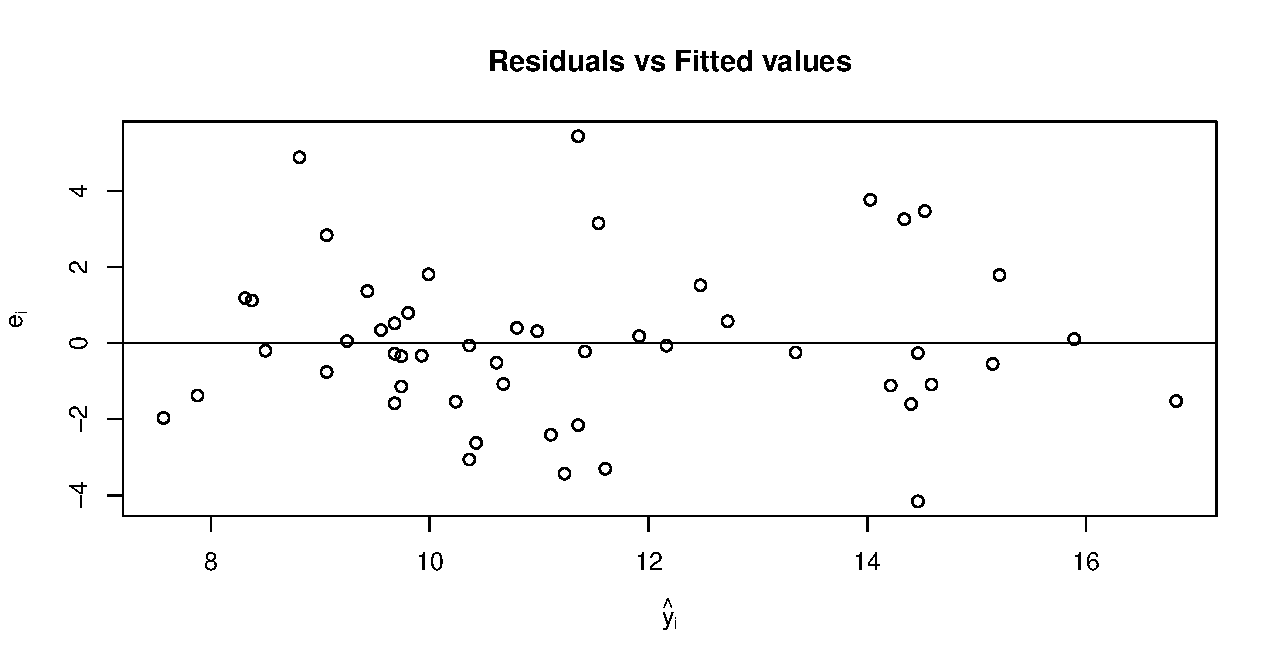
\includegraphics[width=.8\textwidth]{plots/res_fit.pdf}}}
    \item<5->The same plot can be used to check the linearity assumption. \onslide<6->{If the linear model is a good fit, once expects to see the residuals evenly spread on either side of the 0 line.}
\end{itemize}
\end{frame}

\begin{frame}{Graphical Methods: Homogeneity of Variance / Linearity}{Examples of Violations}
\begin{columns}
\pause\begin{column}{.5\textwidth}
\begin{center}
Non-constant variance\\~\\

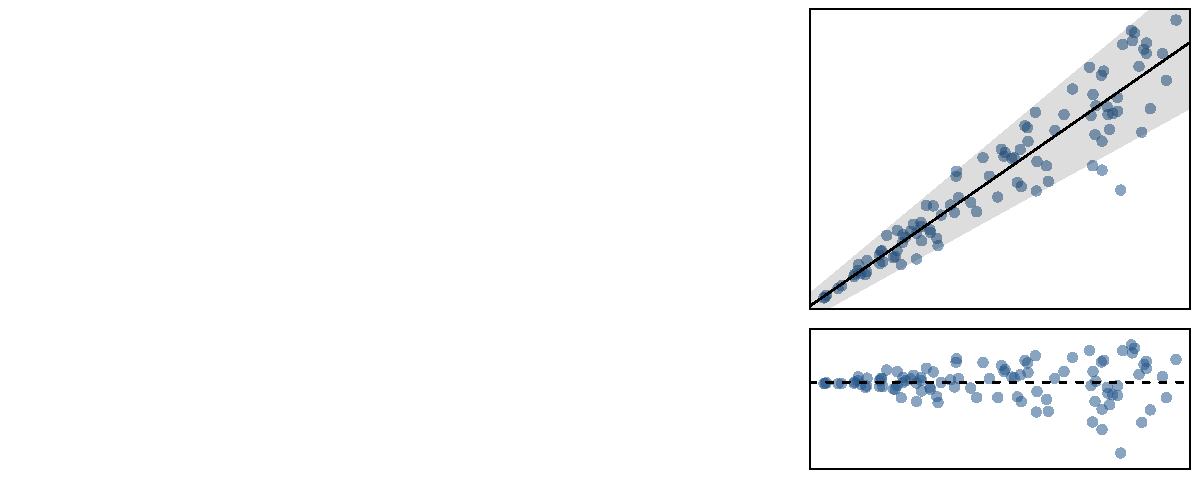
\includegraphics[width=.9\textwidth]{plots/heteroscedastic.pdf}
\end{center}
\end{column}
\pause\begin{column}{.5\textwidth}
\begin{center}
Non-linear relationship\\~\\

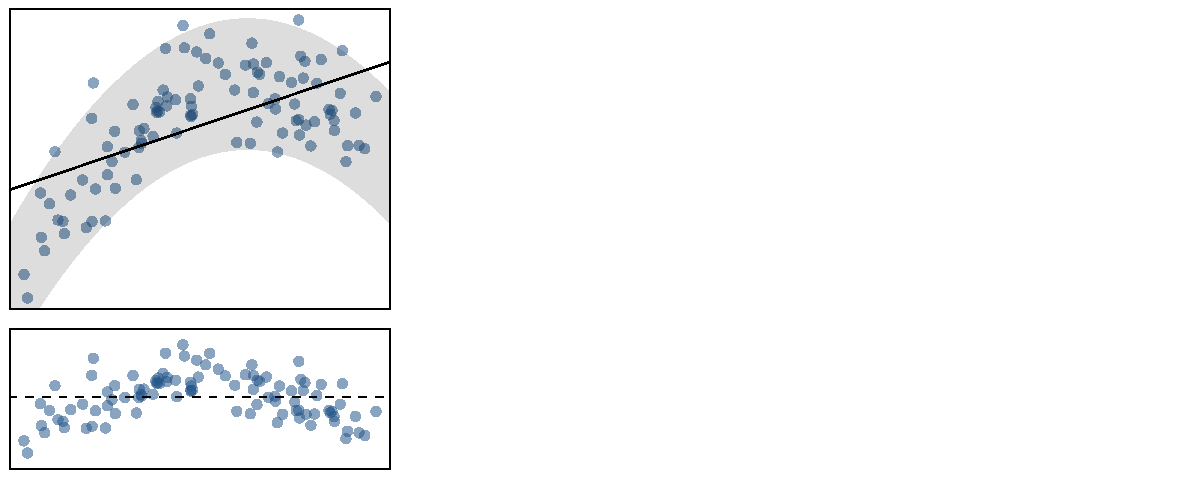
\includegraphics[width=.9\textwidth]{plots/nonlinear.pdf}
\end{center}
\end{column}
\end{columns}
\end{frame}


\begin{frame}{Graphical Methods: Independence}{Time Series Plot of the Residuals}
\begin{itemize}
    \item To check for independence b/w $\epsilon_i$'s, we plot $e_i$ vs $i$.
    \item\pause Independence is graphically checked if there is no discernible pattern in the
plot. \pause I.e., one cannot predict $e_i$ from $e_{<i}$.
\end{itemize}
\pause\begin{center}
    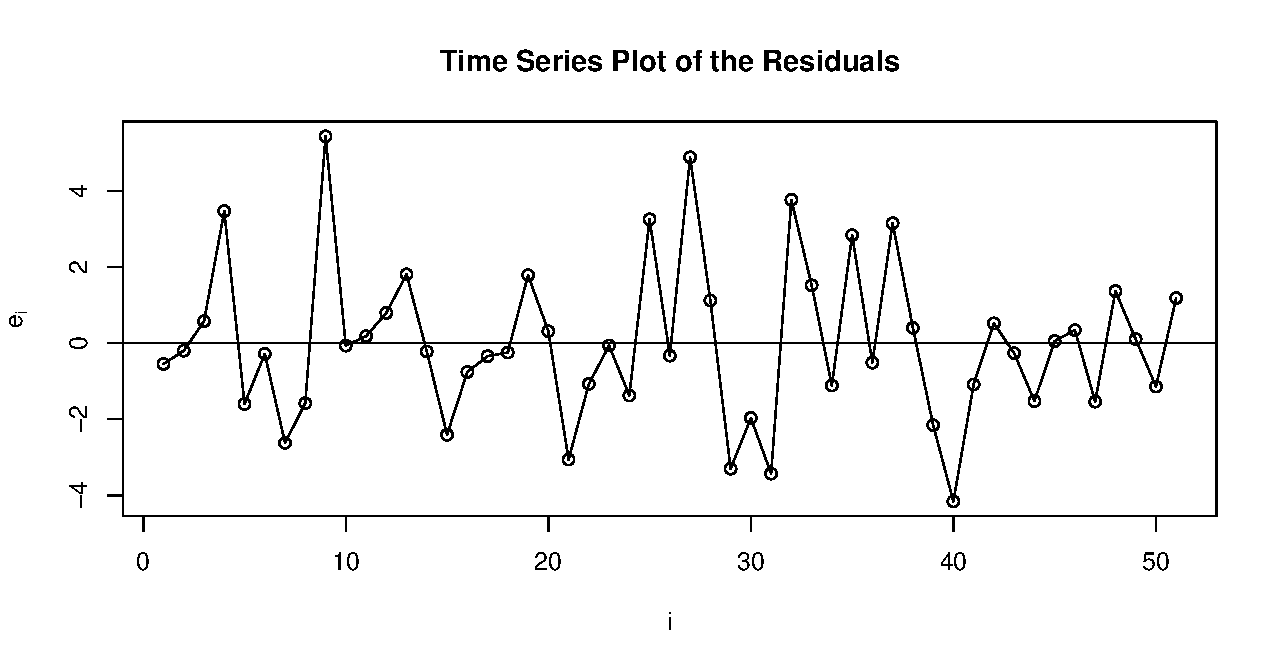
\includegraphics[width=.9\textwidth]{plots/res_ts.pdf}
\end{center}
\vspace{-10pt}
\footnotesize{\color{blue}\url{raw.githubusercontent.com/zh3nis/MATH440/main/chp03/res_plots.R}}
\end{frame}

\subsection{Significance Tests}
\begin{frame}{Runs Test for Independence}
\begin{itemize}
    \item Write out the sequence of $+/-$ signs of the residuals
    \item\pause Count $n_1=\#[e_i\ge0]$, $n_2=\#[e_i<0]$
    \item\pause Count $u=\#\text{runs}$ of positive and negative residuals. \pause What is a \textit{run}? \pause E.g., if we have the following 9 residuals:
    $$
    \underbrace{-}_{1}\underbrace{+++}_{2}\underbrace{--}_{3}\underbrace{+}_{4}\underbrace{--}_{5}
    $$
    then w have $u=5$ runs with $n_1=4$ and $n_2=5$.
    \item\pause Under $\mathrm{H}_0:\,e_i\text{'s are independent}$, the pmf of the r.v. $U$ is
    $$
    p(u)=\begin{cases}
    \frac{2{{n_1-1}\choose{k-1}}{{n_2-1}\choose{k-1}}}{{n_1+n_2\choose n_1}}, &u=2k,\,k\in\mathbb{N}\\
    \frac{{n_1-1\choose k}{n_2-1\choose k-1}+{n_2-1\choose k}{n_1-1\choose k-1}}{{n_1+n_2\choose n_1}},&u=2k+1,\,k\in\mathbb{N}
    \end{cases}
    $$
    \pause And $\text{p-value}=\Pr(U\le u)$. No need to do by hand.
\end{itemize}
\end{frame}

\begin{frame}[fragile]{Runs Test in \texttt{R}}

\begin{small}
\begin{verbatim}
> library(lawstat)
> poverty = read.table("path/to/poverty.txt", h=T, sep="\t")
> my_model = lm(Poverty ~ Graduates, data=poverty)
> re = my_model$residuals
> runs.test(re, plot.it=TRUE)    
	
	Runs Test - Two sided

data:  re
Standardized Runs Statistic = -0.13873, p-value = 0.8897
\end{verbatim}
\end{small}

\centerline{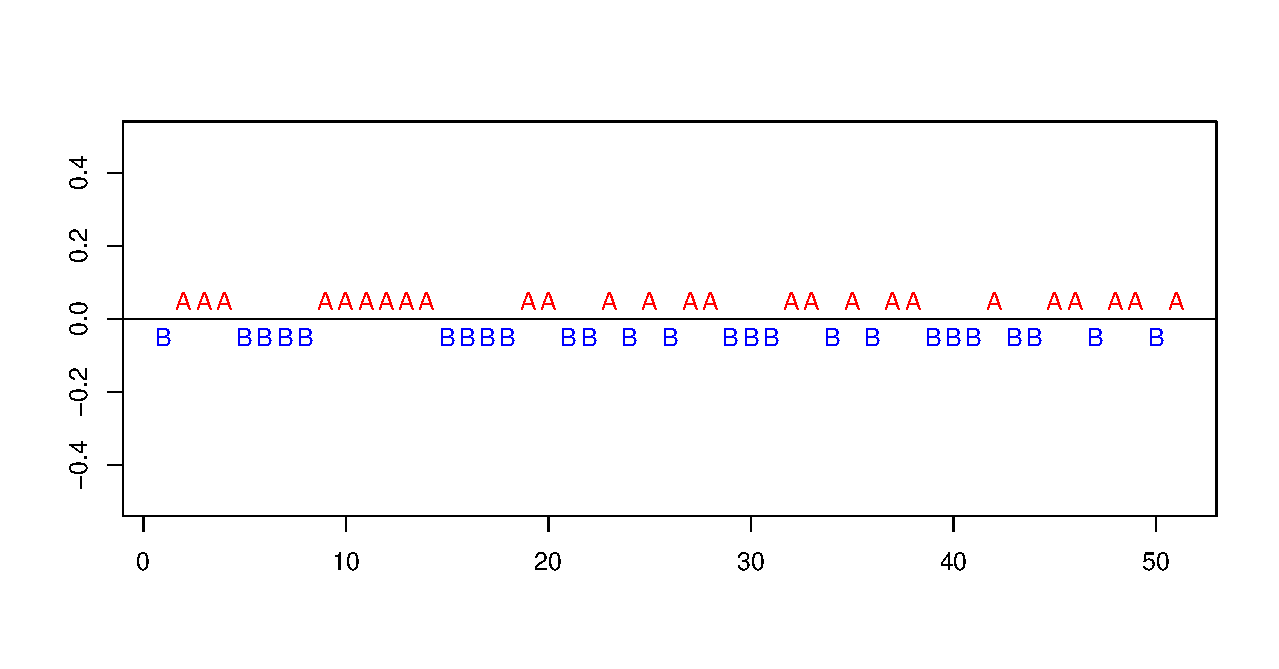
\includegraphics[width=.7\textwidth]{plots/runs.pdf}}

{\color{blue}\url{https://raw.githubusercontent.com/zh3nis/MATH440/main/chp03/runs_test.R}}    
\end{frame}


\begin{frame}{Shapiro-Wilk Test for Normality}
\begin{itemize}
    \item $\mathrm{H}_0:\,e_1,\ldots,e_n\sim\mathcal{N}$
    \item<2->Test statistic
    $$
    W=\frac{\left(\sum_{i=1}^n a_i e_{(i)}\right)^2}{\sum_{i=1}^n(e_i-\bar{e})^2}
    $$
    where
    \begin{itemize}
        \item<3-> $e_{(i)}$ is the $i$th smallest number in the sample
        \item<4-> $(a_1,\ldots,a_n)^\top=\mathbf{a}=\frac{\mathbf{V}^{-1}\mathbf{m}}{\|\mathbf{V}^{-1}\mathbf{m}\|}$
        \item<5->$\mathbf{m}=(m_1,\ldots,m_n)^\top$ is a vector with $m_i=\E[Z_{(i)}]$ where $Z_1,\ldots,Z_n\,\,{\stackrel{\text{iid}}{\sim}}\,\,\mathcal{N}(0,1)$
        \item<6->$\mathbf{V}=\{\Cov[Z_{(i)},Z_{(j)}]\}$
    \end{itemize}
    \item<7->No name for the distribution of $W$ under $\mathrm{H}_0$. Its critical values are calculated through Monte-Carlo simulations.
\end{itemize}
\end{frame}

\begin{frame}[fragile]{Shapiro-Wilk Test in \texttt{R}}
\begin{verbatim}
> poverty = read.table("path/to/poverty.txt", 
                       h=T, sep="\t")
> my_model = lm(Poverty ~ Graduates, data=poverty)
> re = my_model$residuals
> shapiro.test(re)

	Shapiro-Wilk normality test

data:  re
W = 0.96804, p-value = 0.1831    
\end{verbatim}
\pause Hence, FTR normality of the residuals in the Graduation--Poverty example.
\end{frame}

\begin{frame}{Levene's Test for Homogeneity of Variance}
\begin{itemize}
    \item If the response can be split into $t$ distinct groups, the we use Levene's Test for
    $\mathrm{H}_0:\,\sigma^2_1=\ldots=\sigma^2_t$
    \item<2-> If the response is numerical (which is what we have in regression), we can artificially split responses into groups bases on predictor values.
    \item<3-> Test statistic is tedious to calculate and left for software. However,
    $$
    \text{T.S.}\,\,{\stackrel{\mathrm{H}_0}{\sim}}\,\,F_{t-1,n-t}
    $$
    where $t=\#(\text{groups})$, and $n=\#(\text{observations})$. 
    \item<4->The $\text{p-value}=\Pr(F_{t-1,n-t}\ge \text{T.S.})$.
\end{itemize}    
\end{frame}

\begin{frame}[fragile]{Levene's Test in \texttt{R}}{\url{https://raw.githubusercontent.com/zh3nis/MATH440/main/chp03/levene_test.R}}
\begin{small}
\begin{verbatim}
> library(lawstat)
> poverty = read.table("path/to/poverty.txt", 
                       h = T, sep = "\t")
> my_model = lm(Poverty ~ Graduates, data=poverty)
> re = my_model$residuals
> breaks = c(0, 80, 90, 100)
> groups = cut(poverty$Graduates, breaks)
> levene.test(re, groups)

	Modified robust Brown-Forsythe Levene-type test based on the 
	absolute deviations from the median

data:  re
Test Statistic = 0.39829, p-value = 0.6737
\end{verbatim}
\end{small}
\pause FTR homogeneity of variance.
\end{frame}


\section{Remedial Measures}

\begin{frame}{Remedial Measures}
\begin{itemize}
    \item Nonlinear Relation: \pause Add polynomials or transform $x$ and/or $y$ (more emphasis on $x$)
    \item\pause Non-Constant Variance: \pause Weighted Least Squares, transform $x$ and/or $y$, or fit Generalized Linear Model
    \item\pause Non-Independence of Errors: \pause Transform $y$ or use Generalized Least Squares, or fit Generalized Linear Model with correlated errors.
    \item\pause Non-Normality of Errors: \pause Box-Cox transformation, or fit Generalized Linear Model.
    \item\pause Outliers: \pause Robust Regression or Nonparametric Regression
\end{itemize}    
\end{frame}

\begin{frame}{Box-Cox (Power) Transformation}
Transforms the variable $w$ as
$$
w^{(\lambda)}=\begin{cases}
\frac{w^\lambda-1}{\lambda}&\text{if }\lambda\ne0\\
\ln(w)&\text{if }\lambda=0
\end{cases}
$$
\pause It can be applied to the response:
$$
Y_i^{(\lambda)}=\beta_0+\beta_1x_i+\epsilon_i,\qquad\text{with }\epsilon_i\,\,{\stackrel{\text{iid}}{\sim}}\,\,\mathcal{N}(0,\sigma^2)
$$
\pause Or it can be applied to the predictor:
$$
Y_i=\beta_0+\beta_1x_i^{(\lambda)}+\epsilon_i,\qquad\text{with }\epsilon_i\,\,{\stackrel{\text{iid}}{\sim}}\,\,\mathcal{N}(0,\sigma^2)
$$
\pause Software is used to estimate the $\lambda$.
\end{frame}

\begin{frame}{Example: Recalling Items}
In an experiment 13 people are asked to memorize a list of
disconnected items. Asked to recall them at various times up to a week later.\pause
\begin{itemize}
    \item $Y$ --- proportion of items recalled correctly
    \item $x$ --- time, in minutes, since initially memorized the list.
\end{itemize}
\pause\begin{table}
    \centering
    \begin{tabular}{c c c c c c c c}
        \toprule
        $x$ & 1 & 5 & 15 & 30 & 60 & 120 & 240 \\
        $Y$ & 0.84 & 0.71 & 0.61 & 0.56 & 0.54 & 0.47 & .45\\
        \midrule
        $x$ & 480 & 720 & 1440 & 2880 & 5760 & 10080 \\
        $Y$ & 0.38 & 0.36 & 0.26 & 0.20 & 0.16 & 0.08\\
        \bottomrule
    \end{tabular}
\end{table}
\end{frame}

\begin{frame}[fragile]{Box-Cox Transformation in \texttt{R}}

\begin{footnotesize}
\begin{verbatim}
bcPower Transformation to Normality 
            Est Power Rounded Pwr Wald Lwr Bnd Wald Upr Bnd
recall$time    0.0617           0      -0.1514       0.2748

Likelihood ratio test that transformation parameter is equal to 0
 (log transformation)
                           LRT df    pval
LR test, lambda = (0) 0.327992  1 0.56684
\end{verbatim}
\end{footnotesize}
\pause$\Rightarrow$ Log transformation of $x$ seems a good choice. 
\pause \begin{figure}
    \centering
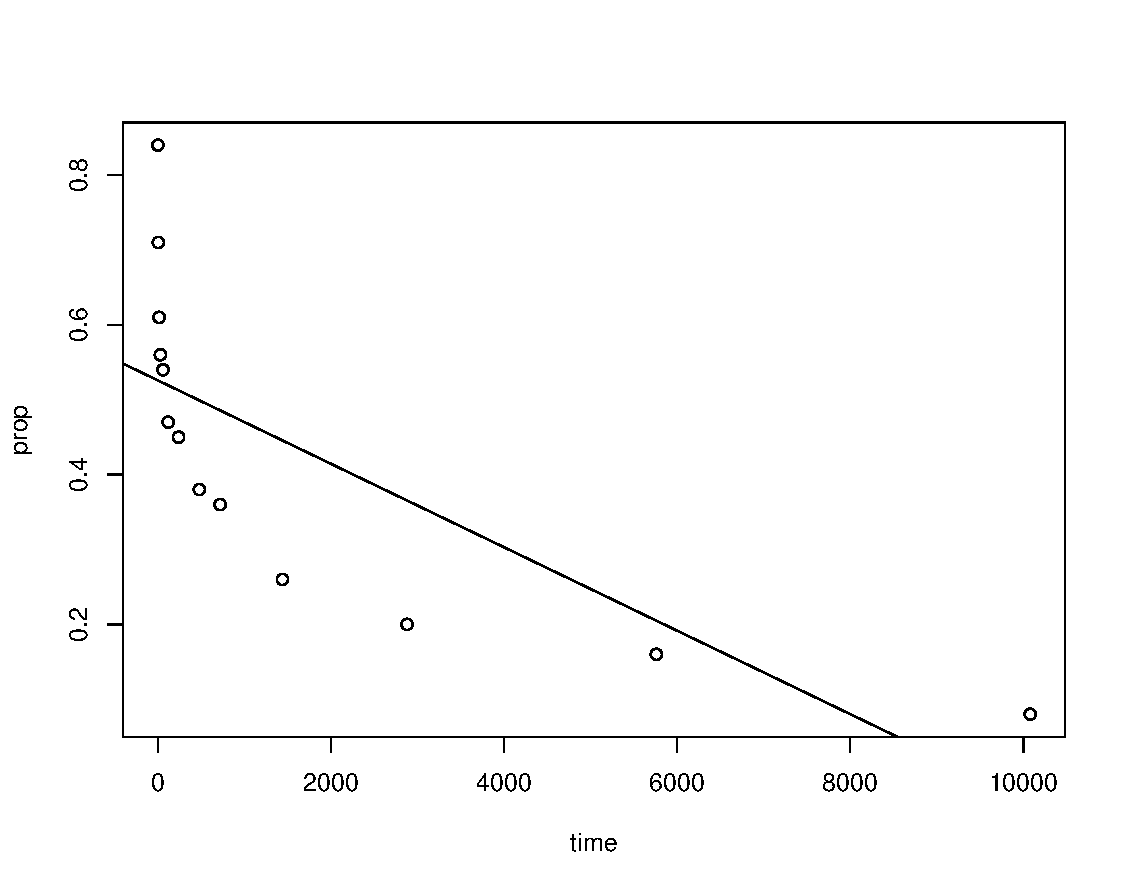
\includegraphics[width=.5\textwidth]{plots/recall_baseline.pdf}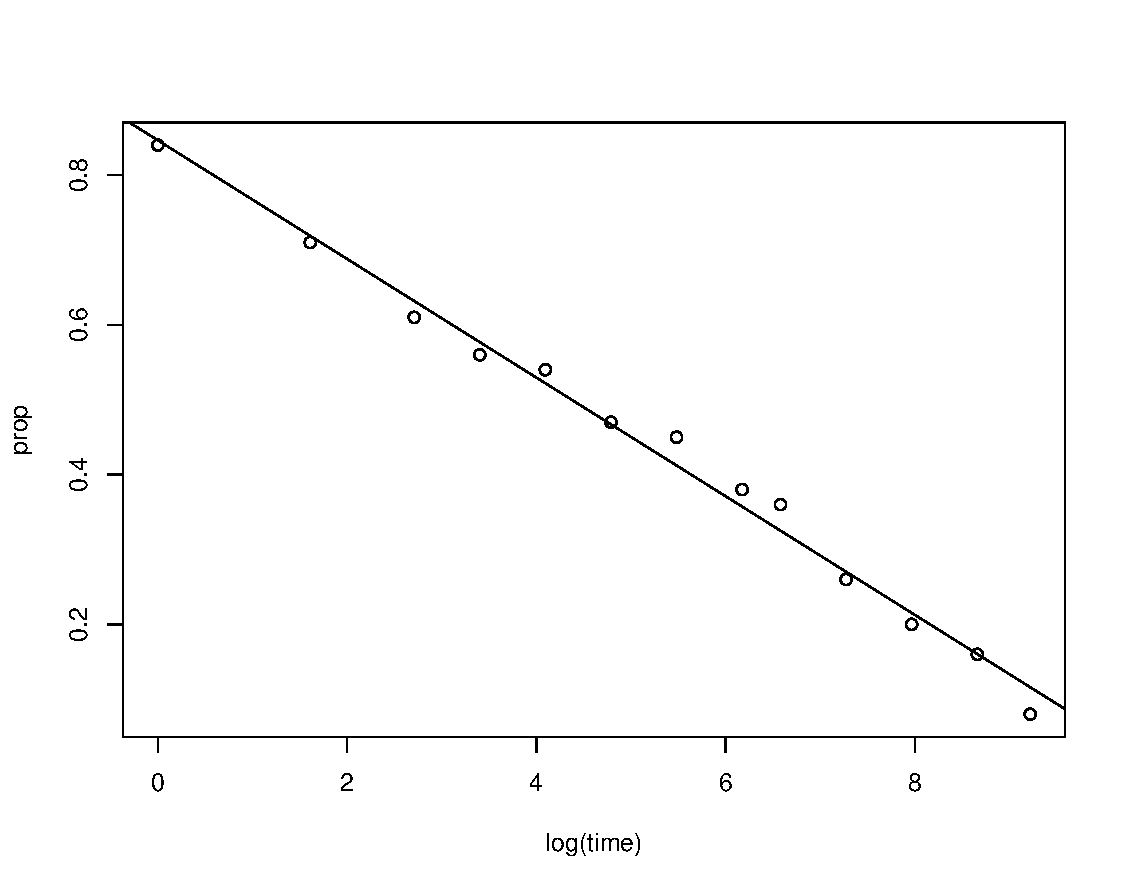
\includegraphics[width=.5\textwidth]{plots/recall_bc.pdf}
    \caption{Left: original data, Right: after log transformation of $x$}
\end{figure}
\end{frame}

\begin{frame}{Graphical Diagnostics for $\hat{Y}_i=\beta_0+\beta_1 x_i$}{\url{https://github.com/zh3nis/MATH440/blob/main/chp03/recall.R}}
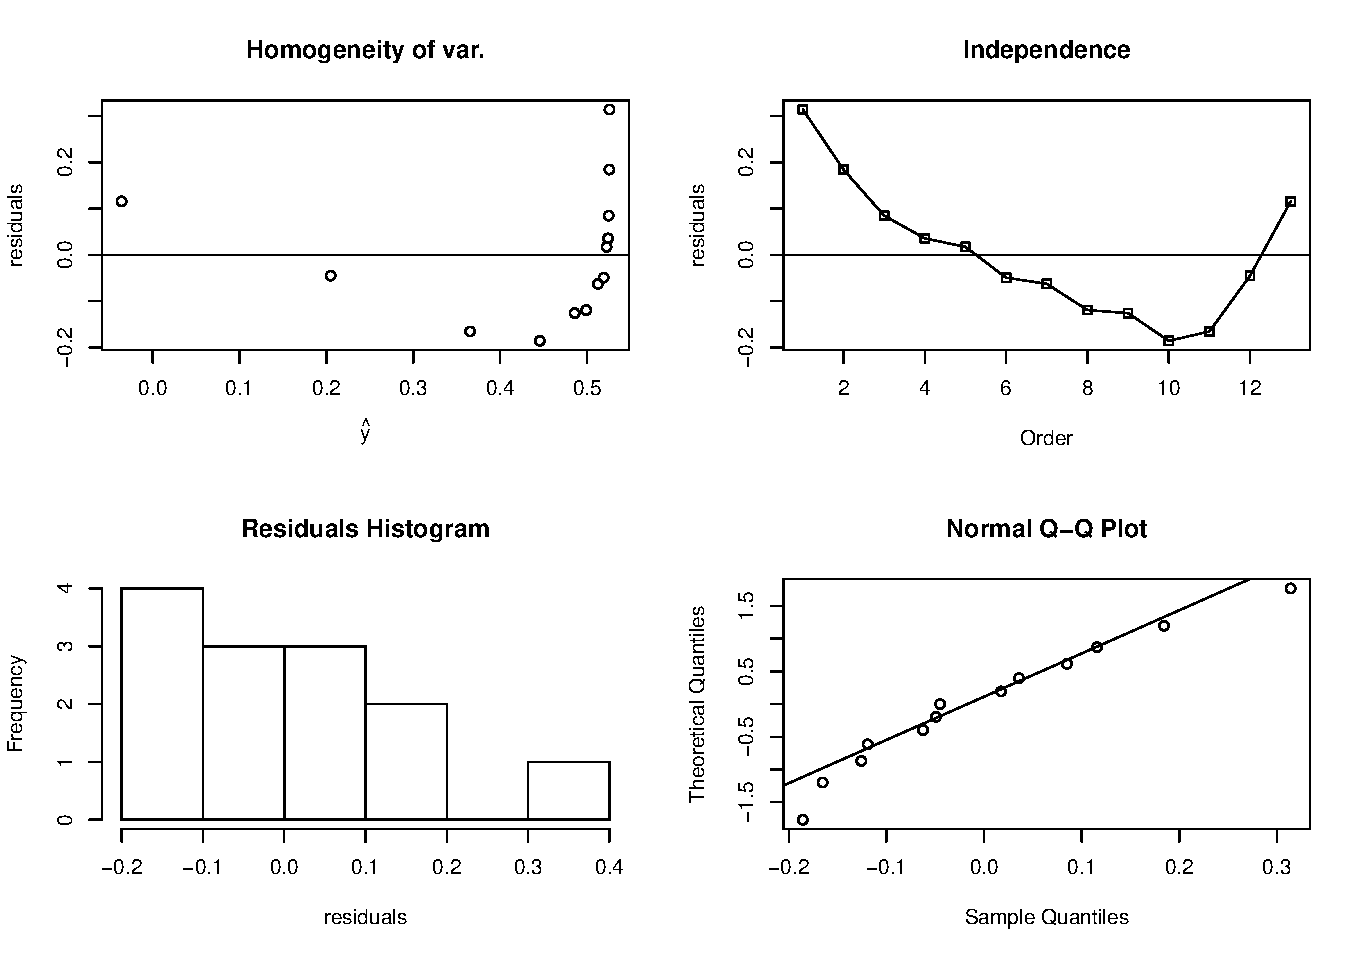
\includegraphics[width=\textwidth]{plots/baseline_diag.pdf}
\end{frame}

\begin{frame}{Graphical Diagnostics for $\hat{Y}_i=\beta_0+\beta_1\ln(x_i)$}{\url{https://github.com/zh3nis/MATH440/blob/main/chp03/recall_boxcox.R}}
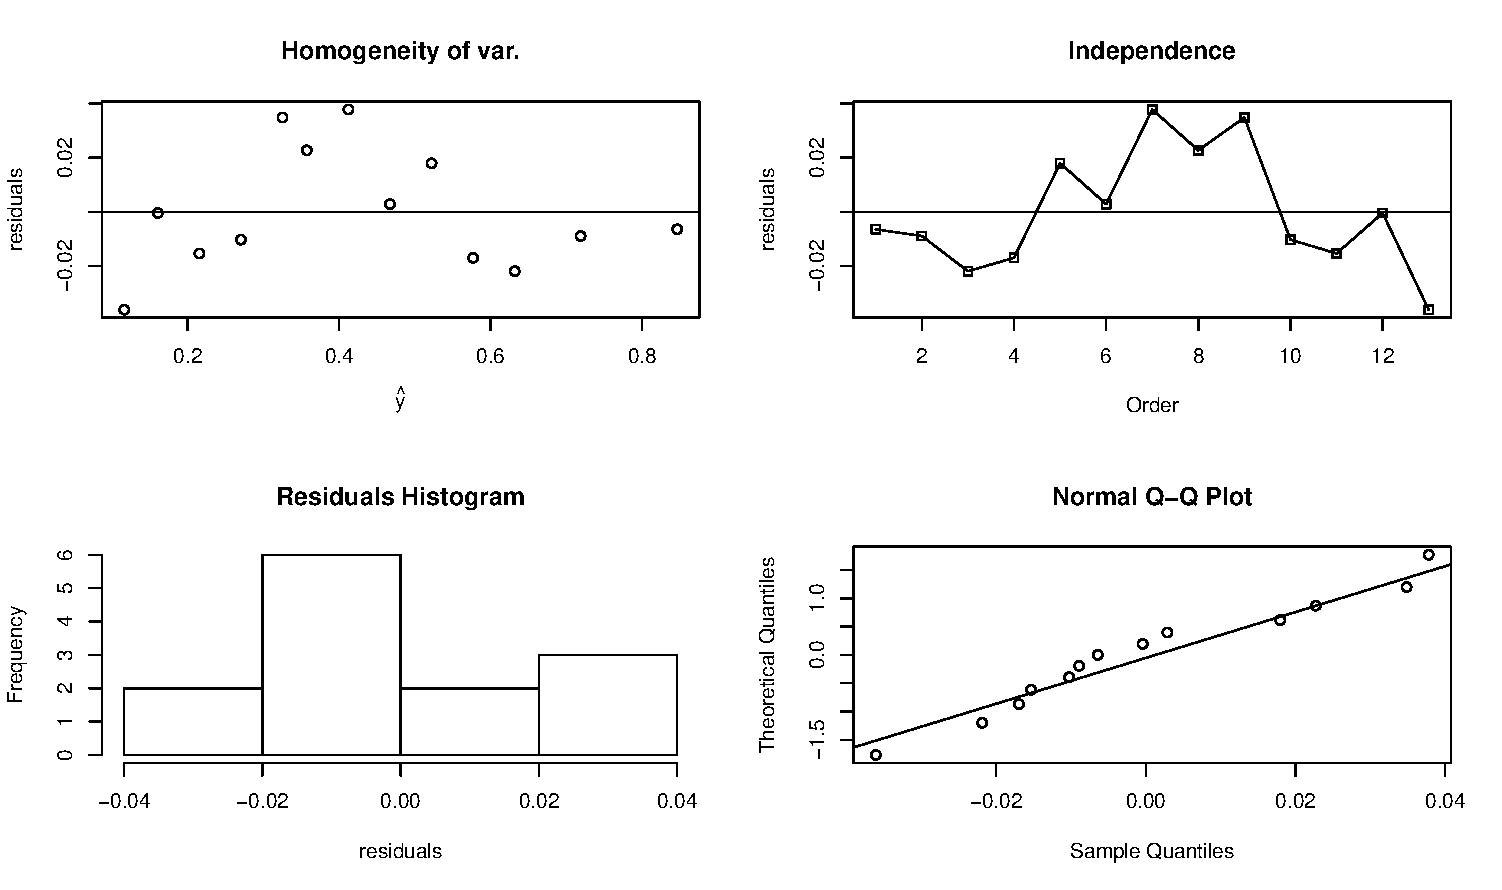
\includegraphics[width=\textwidth]{plots/recall_bc_diag.pdf}
\end{frame}


\end{document}